\section{Návrh architektury}
Před implementací bylo potřeba zvážit dvě různé existující architektury:

\begin{enumerate}
    \item První architektura využívá na serverové straně pouze API, získávání dat a jejich následné zobrazení probíhá pouze klientské straně prostřednictvím jazyka JavaScript. Architektura je zobrazena na diagramu \ref{fig:architecture1}.
    \item Druhá architektura využívá serverovou stranu jak pro API, tak pro získávání dat z~databáze či jiných zdrojů. Architektura je zobrazena na diagramu \ref{fig:architecture2}.
\end{enumerate}

Po domluvě s~vedoucím práce byla vybrána druhá zmiňovaná architektura, a to hlavně z~toho důvodu, že autor již má s~touto architekturou zkušenosti. S~první zmiňovanou se prozatím nesetkal.


\begin{figure}[!h]\centering
    \begin{subfigure}[!h]{0.45\textwidth}
        \centering
        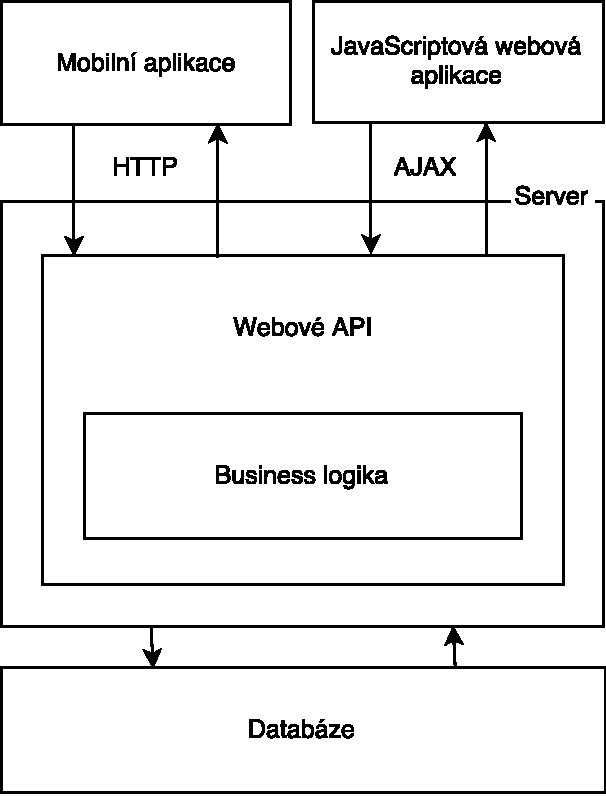
\includegraphics[width=0.8\textwidth]{media/architecture-a.pdf}
        \caption{První uvažovaná architektura aplikace}
        \label{fig:architecture1}
    \end{subfigure}
    \begin{subfigure}[!h]{0.45\textwidth}
        \centering
        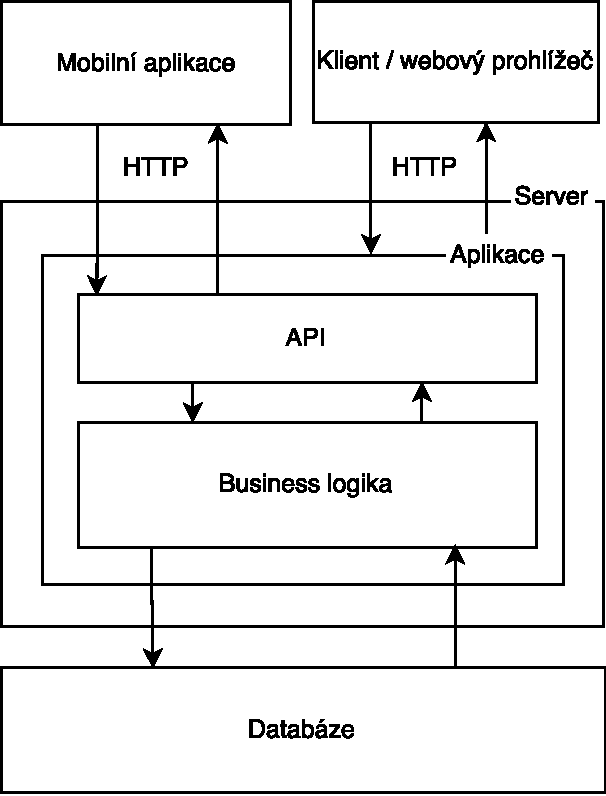
\includegraphics[width=0.8\textwidth]{media/architecture-b.pdf}
        \caption{Druhá uvažovaná architektura aplikace}
        \label{fig:architecture2}
    \end{subfigure}
    \caption{Uvažované architektury aplikace}
\end{figure}